\section{Brain Design} \label{sec:brain}
What follows is a series of descriptions of each of our brain models and what
features they added to the agent's functionality. In general, we wanted to 
start with a brain dead agent, then add to it movement, consumption, 
perception, and eventually judgment. Our figures in this section are used to 
illustrate the elements we have adjusted for each model. The full 
architecture of each model can be seen in appendix~\ref{ap:arch}.

\subsection{Brain 0}
We started from the most simplistic of models: an agent who sits in place until
it dies. It shuns all of its inputs, and uses none of its actuators.

\subsection{Brain 1}

Brain 1 (fig. \ref{fig:brain1}) moves in a straight line and constantly 
activates the agent's eating actuator (i.e. the agent will try to eat anything).

\begin{figure}
\begin{center}
  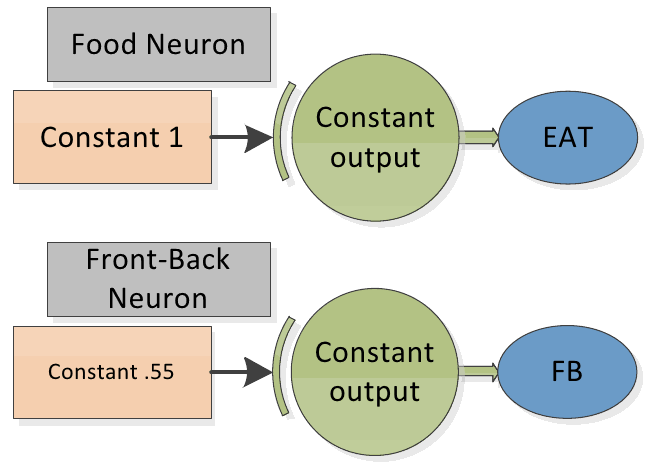
\includegraphics[scale=.3]{img/brain1.png}
  \caption{Active neurons in Brain 1}
  \label{fig:brain1}
\end{center}
\end{figure}

\subsection{Brain 2}

Brain 2 was the first neural network to take advantage of the agent's visual
cortex (fig. \ref{fig:brain2}). Of the 31 eyelets available to the agent, it 
used only the data it received from its center eyelet (eyelet 15). This
neuron instructs the agent to only use its eat actuator when it perceives
intense brightness. 

We caused this behavior by using a single neuron with a step function. 
The neuron was trained by having the agent try to eat at a variety of 
distances and observing the change in its charge. If the charge does not
change, then the brightness threshold is increased.

\begin{figure}
\begin{center}
  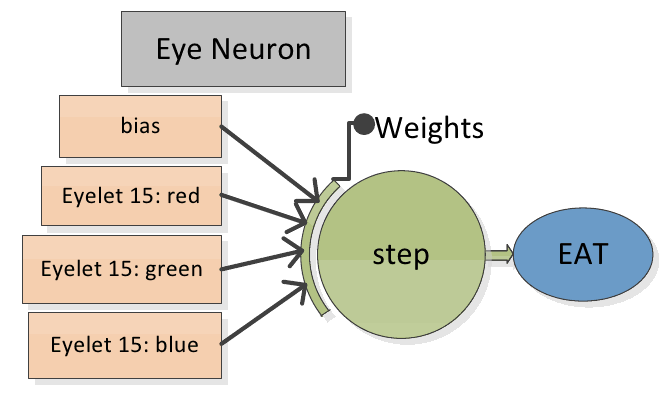
\includegraphics[scale=.3]{img/brain2.png}
  \caption{Brain 2's visual neuron}
  \label{fig:brain2}
\end{center}
\end{figure}

\subsection{Brain 3}

For Brain 4, we actually made two changes. The first was to the
eye neuron, which we changed from a step function to a sigmoid 
(fig. \ref{fig:brain3eye}):

\begin{equation} \label{eq:eyesig}
  \varphi(v) = \frac{\tanh(2v)}{10}
\end{equation}

We made this change because we wanted this model to focus on color. Whereas
our old step function classified \emph{all} objects as ``close enough'' vs. 
``not close enough,'' this new version could classify the color of an object by 
consuming it and comparing the output to the change in energy. Since this 
change 
can only be -0.1, 0, or 0.1, we selected a sigmoid function that would return 
a value within that range. Using a continuous function like equation 
\eqref{eq:eyesig} allows us to compare colors of objects.

\begin{figure}
\begin{center}
  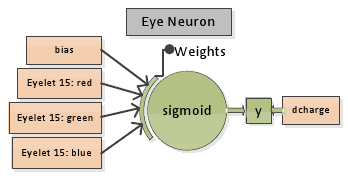
\includegraphics[scale=.7]{img/brain3eye.png}
  \caption{Brain 3's visual neuron}
  \label{fig:brain3eye}
\end{center}
\end{figure}

Our second change was to employ the somatic sensors of the agent
(fig. \ref{fig:brain3touch}). If the agent senses contact on any of its edges, 
it will eat. By using these somatic sensors, we keep our agent from slovenly
gnashing its teeth at every time step.

\begin{figure}
\begin{center}
  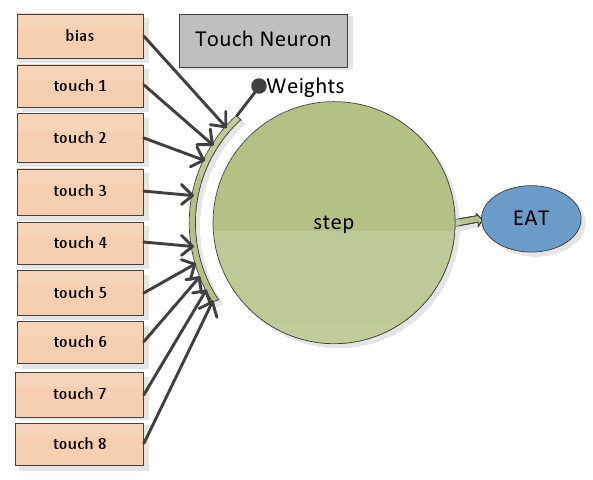
\includegraphics[scale=.5]{img/brain3touch2.png}
  \caption{Brain 3's somatic neuron}
  \label{fig:brain3touch}
\end{center}
\end{figure}

\subsection{Brain 4}

Our mission for Brain 4 was to implement the eyelets into a
winner-take-all network (fig. \ref{fig:brain4}). Each eyelet input is fed 
into two neurons: one \textb{step function} to determine green/not green, and 
another 
which produced the linear summation of each color's intensity. The product of 
these two neurons' outputs is then fed into a 31-element WTA network. All 
neurons in this network connect to a single neuron that controls the rotation 
of the agent, and this neuron has fixed weights coming into it. Each of these 
weights correspond to an angle, which is the direction that eyelet is looking. 
These angles are used to instruct the agent where to turn.

\begin{figure}
\begin{center}
  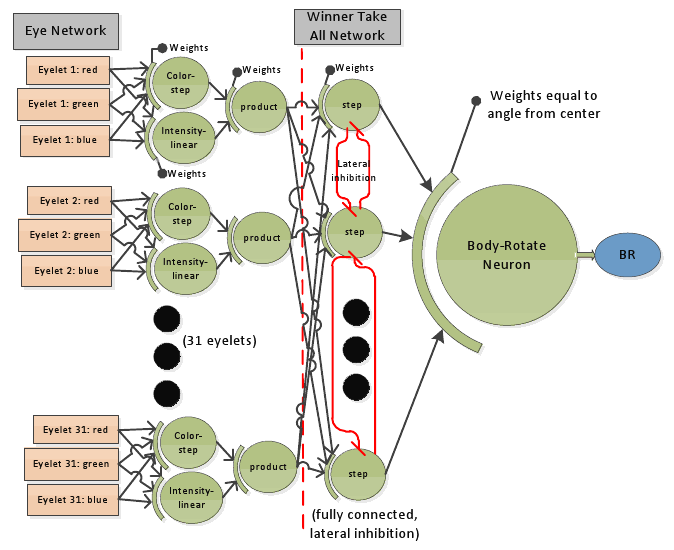
\includegraphics[scale=.62]{img/brain4.png}
  \caption{Brain 4's WTA eyelet network}
  \label{fig:brain4}
\end{center}
\end{figure}

\subsubsection{Waaaait a minute....}
We know what you're thinking. ``Step functions to determine color? But Brain 
3 introduced a sigmoid-based neuron!'' Indeed it is true. Furthermore, Brain
4 exerts no control over the eating actuator either. The reason for this is
that we, as the developers, simultaneously worked on Brains 3 and 4 separately.
Our initial thought was to fuse the two models together and toss the originals 
out. As you will see shortly, we did combine the two. However we kept Brains 
3 and 4 as a demonstration of a sort of evolutionary split in our agent's 
development. So without further ado...

\subsection{Brain 5}
Brain 5 applies the finer-grained sigmoid color neurons from 
fig. \ref{fig:brain3eye} to the augmented WTA network in 
fig. \ref{fig:brain4}. The object consumption is again determined by the 
somatic sensors from fig. \ref{fig:brain3touch}.

\subsection{Brain 6}
At this point in development, we wanted to refine the touch-and-munch nature
of our agent; why would it eat poison when it should know better? In order
to circumvent this greedy, potentially deadly tendency, we added a
color-based neuron to the agent's somatic-gastronomic system 
(fig. \ref{fig:brain6}). The somatic neuron will only fire if there is a
non-zero value \emph{for the ``mouth'' of the agent}. Correspondingly, the
color-based neuron will only fire if an object in contact with it is green.
This is legal to assume, as the agent itself is aware of its own body. It will
never try to eat unless it has made contact with and object, and even then
will only do so if the object is green.

\begin{figure}
\begin{center}
  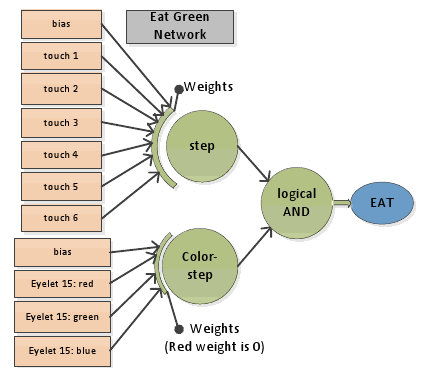
\includegraphics[scale=.7]{img/brain6.png}
  \caption{Brain 6's neural network for eating objects}
  \label{fig:brain6}
\end{center}
\end{figure}

\subsection{Brain 7}
\begin{figure}
\begin{center}
  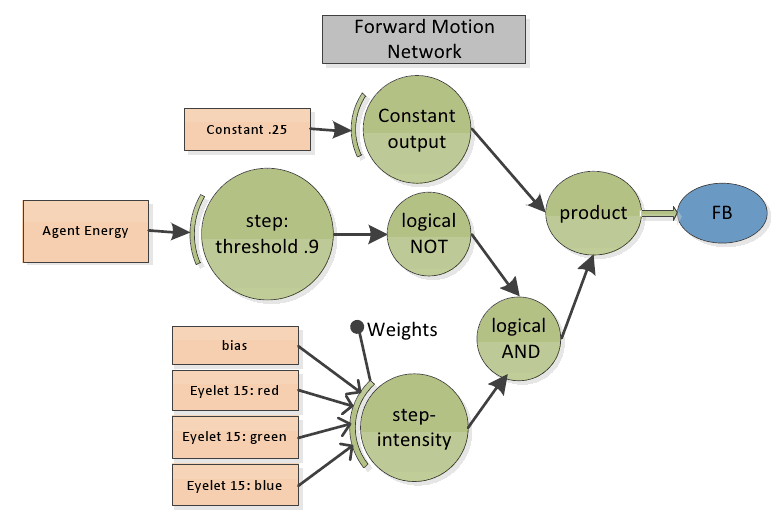
\includegraphics[scale=.5]{img/brain7.png}
  \caption{Brain 7's movement network near food}
  \label{fig:brain7}
\end{center}
\end{figure}

Our seventh and final brain addresses the issue of rationing food supplies in
Flatworld. As previously stated, our agent has a charge/lifespan that is defined
as a real number between 1 and 0, with 1 being a full charge and 0 meaning 
death. Food will increase the agent's charge by \emph{at most} +0.1. Eating 
a food object with a charge of 0.97 brings the agent's charge up to 1, a net
gain of +0.03. In order to get the most out of food objects, our agent
should never eat when it's not hungry. Fig. \ref{fig:brain7} describes our
network to help accomplish this goal.

 Most of the time the agent has the standard propulsion methods as it did in 
other models, fig. \ref{fig:brain7} is put into use under the special 
circumstances that our agent is very close to a food object, but is not hungry.
A constant value describes the forward movement rate (0.25 in this case). At 
every timestep the agent queries its internal charge. While its charge is 
$> 0.9$, the logical NOT will suppress the AND, giving the forward/backward 
actuator a value of $0.25 \times 0 = 0$. Provided the object in question is 
close enough (described by the intensity neuron), when the agent's energy dips
below 0.9, the NOT neuron fires, the AND neuron is satisfied and fires a
non-zero value.
